% !TeX spellcheck = en_US
\documentclass[]{report}
\usepackage[english]{babel}

\usepackage[a4paper, margin=0.9in]{geometry}
\usepackage[utf8]{inputenc}
\usepackage{graphicx} 
\usepackage{float}
\usepackage{lscape}
\usepackage[toc,page]{appendix}
\usepackage{subcaption}


\usepackage{listings}
\usepackage{lmodern}  % for bold teletype font
\usepackage{amsmath}  % for \hookrightarrow
\usepackage{xcolor}   % for \textcolor
%\lstloadlanguages{matlab}

\lstset{
	basicstyle=\ttfamily,
	columns=fullflexible,
%	frame=single,
	breaklines=true,
	postbreak=\mbox{\textcolor{red}{$\hookrightarrow$}\space},
}

% Title Page
\title{Simulation of non-central collision}
\author{Dominik Katszer \\Mateusz Nowotyński}

\def\arraystretch{1.5}

\begin{document}
\maketitle

\section{Aim}
The aim of this project is to simulate collision between 2 balls and edges of board.

\section{Model}
\subsection{Body with body collision}
In order to simulate 2d collision(fig. \ref{fig:collision}) we decided to rotate coordinate system to make x axis parallel to contact angle(fig. \ref{fig:collison_rotated}) therefore reducing problem to single dimension. To get speed components in newly created coordinate system we are using equation \ref{eq:rotate_speed}.
\begin{figure}[h]
\begin{subfigure}{.5\textwidth}
	\centering
	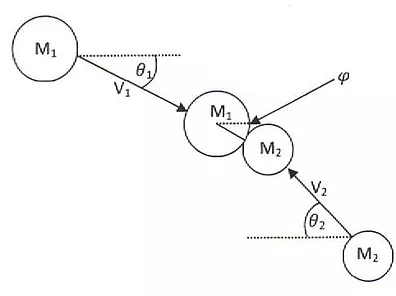
\includegraphics[height=0.8\linewidth]{collision}
	\caption{Draw of simulated collision}
	\label{fig:collision}
\end{subfigure}
\begin{subfigure}{.5\textwidth}
	\centering
	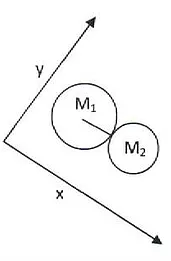
\includegraphics[height=0.8\linewidth]{collision_rotated}
	\caption{Collision with rotated coordinate system}
	\label{fig:collison_rotated}
\end{subfigure}
\caption{}
\end{figure}
\begin{equation}
\begin{aligned}
\label{eq:rotate_speed}
	v_{1xr} &= v_1 \cos(\theta_1 - \varphi) \\
	v_{1yr} &= v_1 \sin(\theta_1 - \varphi) \\
	v_{2xr} &= v_2 \cos(\theta_2 - \varphi) \\
	v_{2yr} &= v_2 \sin(\theta_2 - \varphi) 
\end{aligned}
\end{equation}
After that we can calculate as in one dimension case(eq. \ref{eq:single_dim}) since y component is perpendicular to contact angle.
\begin{equation}
\begin{aligned}
\label{eq:single_dim}
v_{1f} &= \frac{v_1(m_1-m_2) + 2m_2v_2}{m_1+m_2} \\
v_{2f} &= \frac{v_2(m_2-m_1) + 2m_1v_1}{m_1+m_2}
\end{aligned}
\end{equation}
And plugging equations \ref{eq:rotate_speed} into \ref{eq:single_dim} we got \ref{eq:roated_x_components}.
\begin{equation}
\begin{aligned}
\label{eq:roated_x_components}
v_{1fxr} &= \frac{v_1 \cos(\theta_1 - \varphi)*(m_1-m_2) + 2m_2 v_2 \cos(\theta_2 - \varphi)}{m_1+m_2} \\
v_{2fxr} &= \frac{v_2 \cos(\theta_2 - \varphi)*(m_2-m_1) + 2m_1 v_1 \cos(\theta_1 - \varphi)}{m_1+m_2}
\end{aligned}
\end{equation}
Having speed in rotated coordinate system we can un-rotate it to original one with equation \ref{eq:unrotate_speed},
\begin{equation}
\begin{aligned}
\label{eq:unrotate_speed}
v_{1fx} &= v_{1fxr} \cos(\varphi) + v_{1yr} \cos(\varphi + \frac{\pi}{2}) \\
v_{1fy} &= v_{1fxr} \sin(\varphi) + v_{1yr} \sin(\varphi + \frac{\pi}{2}) \\
v_{2fx} &= v_{2fxr} \cos(\varphi) + v_{2yr} \cos(\varphi + \frac{\pi}{2}) \\
v_{2fy} &= v_{2fxr} \sin(\varphi) + v_{2yr} \sin(\varphi + \frac{\pi}{2}) 
\end{aligned}
\end{equation}
therefor receiving final equation \ref{eq:final_equation} used to calculate speed after collision in our simulation.
\begin{equation}
\begin{aligned}
\label{eq:final_equation}
v_{1fx} &= \frac{v_1 \cos(\theta_1 - \varphi)*(m_1-m_2) + 2m_2 v_2 \cos(\theta_2 - \varphi)}{m_1+m_2} \cos(\varphi) + v_1 \sin(\theta_1 - \varphi) \cos(\varphi + \frac{\pi}{2}) \\
v_{1fy} &= \frac{v_1 \cos(\theta_1 - \varphi)*(m_1-m_2) + 2m_2 v_2 \cos(\theta_2 - \varphi)}{m_1+m_2} \sin(\varphi) + v_1 \sin(\theta_1 - \varphi) \sin(\varphi + \frac{\pi}{2}) \\
v_{2fx} &=\frac{v_2 \cos(\theta_2 - \varphi)*(m_2-m_1) + 2m_1 v_1 \cos(\theta_1 - \varphi)}{m_1+m_2} \cos(\varphi) + v_2 \sin(\theta_2 - \varphi) \cos(\varphi + \frac{\pi}{2}) \\
v_{2fy} &= \frac{v_2 \cos(\theta_2 - \varphi)*(m_2-m_1) + 2m_1 v_1 \cos(\theta_1 - \varphi)}{m_1+m_2} \sin(\varphi) + v_2 \sin(\theta_2 - \varphi) \sin(\varphi + \frac{\pi}{2}) 
\end{aligned}
\end{equation}
\subsection{Body with edge collision}
Calculating resulting angle $\gamma$ we were basing on basics of geometry and the law of reflection witch says that the angle of incidence equals the angle of reflection. Original and resulting angle is always related to the horizontal axis. 
\subsubsection{Vertical edges}
\begin{figure}[H]
	\centering
	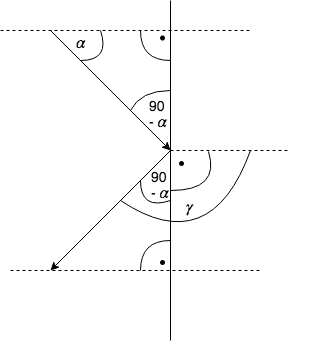
\includegraphics[height=0.4\linewidth]{rightEdge}
	\caption{Bounce from right edge}
	\label{fig:right_edge}
	\end{figure}
	\begin{equation}
\begin{aligned}
\label{eq:right_edge}
\gamma = 90^{\circ} + (90^{\circ} - \alpha) = 180^{\circ} - \alpha
\end{aligned}
\end{equation}
\begin{figure}[H]
	\centering
	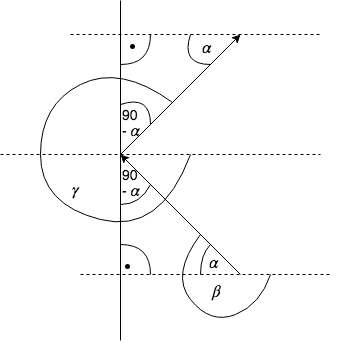
\includegraphics[height=0.4\linewidth]{leftEdge}
	\caption{Bounce from left edge}
	\label{fig:left_edge}
\end{figure}
\begin{equation}
\begin{aligned}
\label{eq:left_edge}
\alpha & = \beta - 180^{\circ}\\
\gamma & = 270^{\circ}+(90^{\circ}-\alpha) = 360^{\circ} - \alpha \\
\gamma & = 360^{\circ} - \beta + 180^{\circ} = 180^{\circ} - \beta
\end{aligned}
\end{equation}
Taking both figures into consideration we can conclude that it does not matter from which edge ball will bounce, it can be always calculated from the same equation.
\begin{equation}
\begin{aligned}
\label{eq:vertical_edge}
\gamma = 180^{\circ} - \beta
\end{aligned}
\end{equation}
\begin{align*}
\text{where} \\
\beta -& \text{~~Value of angle before edge collision} \\
\gamma -& \text{~~Value of angle after edge collision}
\end{align*}
\subsubsection{Horizontal edges}
\begin{figure}[H]
	\centering
	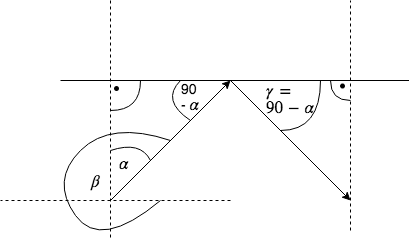
\includegraphics[height=0.4\linewidth]{topEdge}
	\caption{Bounce from top edge}
	\label{fig:top_edge}
	\end{figure}
\begin{equation}
\begin{aligned}
\label{eq:top_edge}
\alpha &= \beta - 270^{\circ} \\
\gamma &= 90^{\circ} - \alpha \\
\gamma &= 90^{\circ} + 270^{\circ} - \beta \\
\gamma &= 360^{\circ} - \beta
\end{aligned}
\end{equation}
\begin{figure}[H]
	\centering
	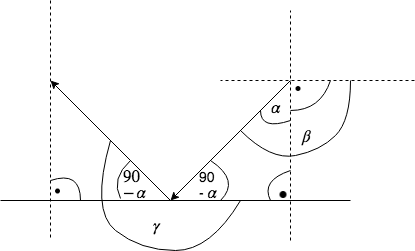
\includegraphics[height=0.4\linewidth]{bottomEdge}
	\caption{Bounce from bottom edge}
	\label{fig:bottom_edge}
\end{figure}

\begin{equation}
\begin{aligned}
\label{eq:bottom_edge}
\alpha &= \beta - 90^{\circ} \\
\gamma &= 180^{\circ} + 90^{\circ} - \alpha \\
\gamma &= 270^{\circ} + 90^{\circ} - \beta \\
\gamma &= 360^{\circ} - \beta 
\end{aligned}
\end{equation}
In this scenarios, we can observe the very similar thing as it was discovered in vertical edges. We can calculate resulting angle using the same equation for bouncing from the top and bottom edge.
\begin{equation}
\begin{aligned}
\label{eq:horizontal_edge}
\gamma = 360^{\circ} - \beta
\end{aligned}
\end{equation}
\begin{align*}
\text{where} \\
\beta -& \text{~~Value of angle before edge collision} \\
\gamma -& \text{~~Value of angle after edge collision}
\end{align*}
\section{Implementation}
Simulation is implemented in JavaScript using p5js library to render results on canvas. Each ball is moved each frame based on their current velocity,
\begin{lstlisting}
move() {
	this.x = this.x + this.vx;
	this.y = this.y + this.vy;
}
\end{lstlisting}
in every frame we check if two balls intersects with each other
\begin{lstlisting}
intersects(other) {
	let distanceBetweenBalls = dist(this.x, this.y, other.x, other.y);
	return (distanceBetweenBalls < this.r + other.r);
}
\end{lstlisting}
and new velocities are calculated
\begin{lstlisting}
collide(other) {
	let v1 = Math.sqrt(this.vx*this.vx + this.vy*this.vy);
	let v2 = Math.sqrt(other.vx*other.vx + other.vy*other.vy);
	let a1 = this.getAngle();
	let a2 = other.getAngle();
	let ca = this.contactAngle(other);
	let m1 = this.m;
	let m2 = other.m;
	
	let n = v1*Math.cos(a1 - ca)*(m1-m2) + 2 * m2 * v2 * Math.cos(a2 - ca);
	let d = m1 + m2;
	
	
	this.new_vx = n * Math.cos(ca) / d + v1 * Math.sin(a1 - ca) * Math.sin(ca);
	this.new_vy = n * Math.sin(ca) / d + v1 * Math.sin(a1 - ca) * Math.cos(ca);
}
\end{lstlisting}
\newpage
What is more, every time we check if collision with some edge happen.
\begin{lstlisting}
    isOutOfBoardEdge(pos, boardEdgeSize) {
        return pos + this.r >= boardEdgeSize || pos - this.r <= 0;
    }

    bounceFromBoardEdge(cvnWidth, cvnHeight){
        if(this.isOutOfBoardEdge(this.x, cvnWidth)){
            this.updateAfterBounceFromEdge(Math.PI - this.getAngle());
        }
        if(this.isOutOfBoardEdge(this.y , cvnHeight)){
            this.updateAfterBounceFromEdge(2*Math.PI - this.getAngle());
        }
    }
\end{lstlisting}

First \verb!if! statement check if center position of considered ball plus its radius exceed canvas horizontally. In other words, it checks if this ball collides with vertical edges. 
 
Second \verb!if! statement works very similarly but checks eventual collisions with horizontal edges.

In both cases, when they happen, movement direction is changed basing on resulting angle after bouncing.

\begin{lstlisting}
    updateAfterBounceFromEdge(resultedAngle) {
        let velocity = Math.sqrt(Math.pow(this.vx,2) + Math.pow(this.vy,2));
        this.vx = this.calculateVx(velocity, resultedAngle);
        this.vy = this.calculateVy(velocity, resultedAngle);
    }
    calculateVx(velocity, angle) {
        return  velocity * Math.cos(angle);
    }
    calculateVy(velocity, angle) {
        return  velocity * Math.sin(angle);
    }

\end{lstlisting}
\section{Conclusion}
This simulation achieved target goal. Non-central collision of two balls is presented in a clear way by preserving physical principles such as the principle of energy conservation and the law of reflection. We have not taken into consideration the friction forces in order to simplify simulation and focus mainly on collision. Thanks to the fact that it is implemented in javascript it does not require specific prepared environment. It just can be opened in any web-browser where each ball can be placed everywhere we want and mass of each ball can be set. 

\end{document}          
